\documentclass[12pt]{article}
\usepackage{amsmath, amssymb, amsbsy}
\usepackage{graphicx, subfigure}
\usepackage[margin=1in,nohead]{geometry}
\usepackage{siunitx}
\usepackage{url}
\usepackage{cite}
\usepackage{algorithm}
\usepackage{algpseudocode}

\makeatletter
\def\BState{\State\hskip-\ALG@thistlm}
\makeatother

\setlength{\parindent}{0pt}
\setlength{\parskip}{12pt}

\renewcommand\algorithmicthen{}
\renewcommand\algorithmicdo{}

\newcommand{\uv}[1]{\ensuremath{{\hat{#1}}}} % for unit vector
\newcommand{\abs}[1]{\left| #1 \right|} % for absolute value
\newcommand{\avg}[1]{\left< #1 \right>} % for average
\let\underdot=\d % rename builtin command \d{} to \underdot{}
\renewcommand{\d}[2]{\frac{d #1}{d #2}} % for derivatives
\newcommand{\dd}[2]{\frac{d^2 #1}{d #2^2}} % for double derivatives
\newcommand{\pd}[2]{\frac{\partial #1}{\partial #2}} % for partial derivatives
\newcommand{\pdd}[2]{\frac{\partial^2 #1}{\partial #2^2}} % for double partial derivatives
\newcommand{\pdc}[3]{\left( \frac{\partial #1}{\partial #2}
\right)_{#3}} % for thermodynamic partial derivatives
\newcommand{\ket}[1]{\left| #1 \right>} % for Dirac bras
\newcommand{\bra}[1]{\left< #1 \right|} % for Dirac kets
\newcommand{\braket}[2]{\left< #1 \vphantom{#2} \right|\left. #2 \vphantom{#1} \right>} % for Dirac brackets
\newcommand{\matrixel}[3]{\left< #1 \vphantom{#2#3} \right|#2 \left| #3 \vphantom{#1#2} \right>} % for Dirac matrix elements
\newcommand{\grad}[1]{\gv{\nabla} #1} % for gradient
\let\divsymb=\div % rename builtin command \div to \divsymb
\renewcommand{\div}[1]{\gv{\nabla} \cdot #1} % for divergence
\newcommand{\curl}[1]{\gv{\nabla} \times #1} % for curl
\let\baraccent=\= % rename builtin command \= to \baraccent
\newcommand{\partder}[2]{\frac{\partial #1}{\partial #2}}
\newcommand{\material}[2]{\frac{D #1}{D #2}}
\newcommand{\tensor}[1]{\bar{#1}}
\newcommand{\tensplus}[3]{\tensor{#1}_{#2}^{#3}}

\title{Implementation of 1-D Vascular Model using Structured Tree Outflow Conditions}
\author{Alex Baelde, Adam Updegrove, Debanjan Mukherjee}

\begin{document}
\maketitle
\section{Introduction}
Using the paper reviewed in Journal Club, we attempted to implement the Structured Tree Outflow conditions for a 1-D Vascular Model presented by Olufsen~\cite{structuredtree}. The 1-D model presented by Olufsen outlines a finite difference scheme for solving the Navier-Stokes equations; as such, we used this approach for implementation of our 1-D model. We will briefly outline the purpose of using a Structured Tree model and the theory behind this implementation.%as well as potential points of error in the discretization.
We will then describe the process taken in implementing this code along with some issues encountered along the way. We will discuss the current state of our code as well as display some preliminary results of our implementation. Lastly, we will talk about a small study investigated using Olufsen's code. 

\section{Theory}

\subsection{Why Structured Tree}

Modeling the human body, in the current state of being, is a complex and difficult process. Large 3-D models that account for large portions of the human vasculature take immense amounts of computation time to solve for the flow within the body. On the other hand, smaller models that take into account the rest of the body as a set resistance or circuit (lumped parameter models) cannot accurately resolve the physiological wave reflections in the human vasculature~\cite{structuredtree}. The Structured Tree 1-D model lies somewhere in between the two complexities. It is a 1-D model, so computational time is significantly decreases; in addition, the wave reflections of the human vasculature are captured because the impedance of the human body is modeled as an impedance based on frequency of the downstream vessels (The Structured Tree). It is important to note that the formation of this tree, specifically the root impedance, can have an effect on the solution. The effect of  a change in root impedance is investigated later in the paper.

\subsection{Inflow}

For the inflow into the 1-D model, a mathematical model fit to measured data was used to represent the pulses of the human cardiac cycle. This mathematical model is described in Olufsen's thesis~\cite{olufsenthesis}.This is imposed as an initial condition in the first cardiac period. The following plot is produced to describe the velocity for the inlet.

\begin{figure}[ht]
	\centering
	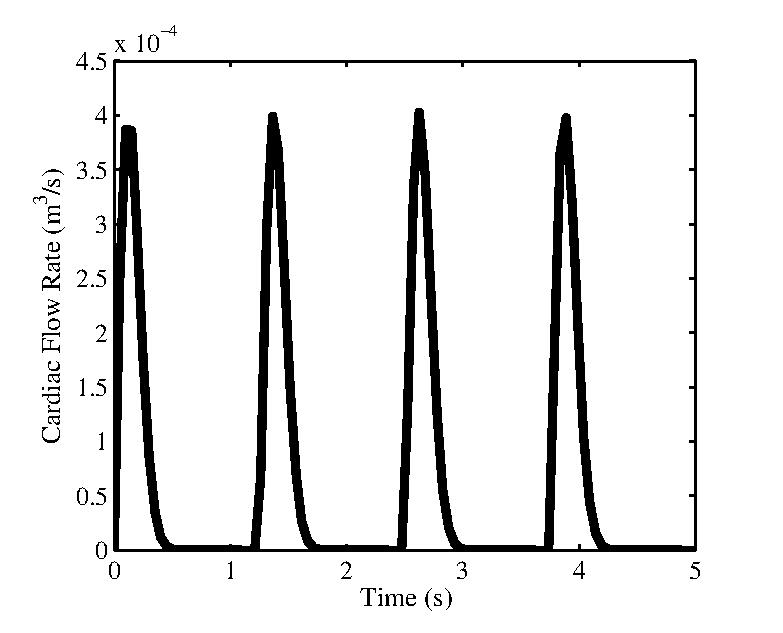
\includegraphics{inflow}
	\label{inflower}
	\caption{The inflow profile from measured data in $m^3/s$. The curve is measured at the upper ascending aorta using magnetic resonance.}
\end{figure}


\subsection{Interior}
As is commonly the case, blood is modeled as an incompressible, newtonian fluid. The navier-stokes equation of motion are therefore applied to the fluid. Starting with a simplified version of continuity, we get Equation~\eqref{continuity}, and the simplified conservation of momentum in the x direction we get Equation~\eqref{consxmomentum}.

\begin{equation}
	\label{continuity}
	\partder{A}{t} + \partder{q}{x} = 0
\end{equation}

\begin{equation}
	\label{consxmomentum}
	\partder{q}{t} + \partder{}{x}\Bigg(\frac{q^2}{A}\Bigg) + \frac{A}{p}\partder{p}{x} = -\frac{2R\pi \nu q}{\delta A}
\end{equation}

For implementation of these non-linear equations, a Two-Step Lax-Wendroff (Richtmyer) scheme is used. Equations~\ref{continuity} and \ref{consxmomentum} can be written in the following form:

\begin{equation} 
	\label{discrete1}
	\partder{}{t} \tensor{U} + \partder{}{x} \tensor{R}(\tensor{U}) = \tensor{S}
\end{equation}

This equation is than discretized into the two equations two be solved over the interior domain. 

\begin{enumerate}
	\item
	\begin{equation}
		\label{bigu1}
		\tensplus{U}{j}{T+1} = \tensplus{U}{j}{T} - \frac{k}{h} \Bigg(\tensplus{R}{j+1/2}{T+1/2} - \tensplus{R}{j-1/2}{T+1/2} \Bigg) + \frac{k}{2} \Bigg(\tensplus{S}{j		+1/2}{T+1/2} + \tensplus{S}{j-1/2}{T+1/2} \Bigg)
	\end{equation}
	
	\item
	\begin{equation}
		\label{bigu2}
		\tensplus{U}{j}{T+1/2} = \frac{\tensplus{U}{j+1/2}{T} + \tensplus{U}{j-1/2}{T}}{2} + \frac{k}{2h} \Bigg(-\tensplus{R}{j+1/2}{T} - \tensplus{R}{j-1/2}{T} \Bigg)  		+ \frac{k}{4} \Bigg(\tensplus{S}{j+1/2}{T} + \tensplus{S}{j-1/2}{T} \Bigg)
	\end{equation}
\end{enumerate}

In terms of implementing the equation, the very broad algorithm can be viewed to help describe the process:

\begin{algorithm}
\caption{Implementation}\label{euclid}
\begin{algorithmic}[1]
\State Set up problem based on user input.
\State Solve for impedance tree.
\For{$i = 1 $ : Number of Cardiac Periods}
	\If{$1^{st}$ Cardiac Period}
		\State Apply the inflow condition.
	\Else
		\State Use the flow from previous period.
	\EndIf
	\For{$j = 1$ : Time in Cardiac Period}
		\For{$k = 1$ : Number of Nodes in Domain}
			\State Solve equations \ref{bigu1} and \ref{bigu2} for each component of the $\tensor{U}$, $\tensor{R}$, and $\tensor{S}$ vectors.
		\EndFor
	\State Apply the outflow condition.
	\EndFor
\State Save the Period Information.
\EndFor
\end{algorithmic}
\end{algorithm}

\subsection{Outflow}
Our implementation of the structured tree actually varies slightly from Olufsen's implementation. In her code, Olufsen runs through each vessel individually and calculates the radius of the vessel based on Equation~\eqref{radius}. She retains no structure of the vessels within the tree and recalculates all this information for each structured tree.

\begin{equation}
	\label{radius}
	(r_0)_(n,k) = R_{root} \alpha^k\beta^{n-k}
\end{equation}

where $\alpha$ and $\beta$ are constants that describe the reduction and asymmetry of the vascular tree. $n$ is the number of total generations of the tree and $k$ is the current generation. She the calculates the corresponding impedance in the same recursive step and returns the total tree impedance at each corresponding frequency. 

Our algorithm, however, is based off of a class that we have defined in order to retain information about the tree. We iterate through each generation of the tree and develop two daughters from each branch by applying $\alpha$ and $\beta$ separately to each member. In the end, we have an array that describes the breakdown of this entire tree with the following format:

\begin{equation}
	\begin{bmatrix}
		Daughter \: 1 \; & Daughter \: 2 \; & Parent \; & Radius 
	\end{bmatrix}
\end{equation}

The Inverse Fourier Transform of the impedance is taken in order to get the impedances as a function of time. These impedances are then used to couple the outflow condition to the solution by either using another Lax-Wendroff discretization or a method of Positive Characteristics. This was actually something that is extremely different between Olufsen's thesis and her code, and actually became a big turning point in getting our code working. In her thesis, she states that a Lax-Wendroff method must also be used at the outflow in order to guarantee $2^{nd}$ order accuracy; however, she doesn't use this method and instead uses a method of positive characteristics. We implemented the method of positive characteristics as an alternative to the Lax-Wendroff discretization to provide an alternate, more reduced approach.

\begin{figure}[ht]
	\centering
	\label{characteristicplot}
	\includegraphics[width=3.5in]{characterplot}
	\caption{At the right boundary, or the outlet, the source vector $\tensor{S}$, and the $\tensor{R}$ converge at point $Q$ using the method of positive characteristics.~\cite{olufsenthesis}}
\end{figure}

 \begin{equation}
 	\label{characteristics}
 	\Gamma_{+/-}\; : A_Q - A_{R/S} + \frac{Q_Q - Q_{R/S}}{-(Q_{R/S}/A_{R/S}) + C_R} = H_{R/S}^{+/-} \Delta t
\end{equation}

\section{Methods and Results}
\subsection{Our Implementation}
For future ease of use, Matlab was used as the coding interface. This will allow future students and lab members to easily use the code and either experiment or make modifications to the code. The only down side to this is the fact that the code runs much slower than if it were implemented in fortran or c. The drastic effect of computation time is seen by the mere seconds it takes for Olufsen's code to finish compared to the ten minutes or so it takes for the Matlab implementation. With our code, we are at a point where the code runs, but only for problems of very carefully specified parameters. In addition, for debugging purposes, we set up the code to be able to use a resistance boundary condition to try to isolate whether the problem was in the interior of the domain or while implementing the boundary conditions. This helped to figure out separate issues in the code, as there seemed to be problems with both. The code now works for certain test cases using a resistance boundary condition, but \textit{interesting} things are happening for other problems. The following problem is run on a tube with a length of 100 cm and a radius of 1 cm. This case was run in order to try to compare with a test case run in Olufsen's paper. Olufsen runs a test case using a resistance boundary condition on a tube of equal length, but with decreasing radius. Her radius starts at 0.5 cm and decreases to 0.25 cm. The reason we have not run this exact test size is because the code cannot seem to handle the change in radius at this point. This is likely the reason for the discrepancy in both flow and pressure values. The profiles, however, look fairly similar and can be compared. The results of two problems are shown below:

\begin{figure}[ht]
	\centering
	\includegraphics[width=6in]{pplot}
	\label{ours}
	\caption{Surface plot of the pressure along the tube for one cardiac period. \textbf{Left:} Plot from Olufsen's thesis during fourth cardiac cycle. \textbf{Right:} Plot from our implementation during fourth cardiac cycle. Our implementation seems to have less of a dicrotic notch after the peak pressure in the cardiac cycle.}
\end{figure}

\begin{figure}[ht]
	\centering
	\includegraphics[width=6in]{qplot}
	\label{ours}
	\caption{Surface plot of the flow in $cm^3/s$ along the tube for one cardiac period. \textbf{Left:} Plot form Olufsen's thesis during fourth cardiac cycle. \textbf{Right: } Plot from our implementation during fourth cardiac cycle. Our implementation retains the similar profile, but again, the slight notch in the curve is less visible in our implementation.}
\end{figure}

\pagebreak

\subsection{Olufsen Implementation}
As you know, we were able to get in touch with Olufsen, and she generously sent us her code via e-mail. We were able to compile, run, and post process her code. Because our code is not to the point where we can investigate some of the things we were hoping to, we modified her code in certain ways to display some interesting things. We investigated the following things:

\begin{itemize}
	\item
		Effect of decreasing the cardiac period
	\item
		Blocking flow in certain arteries (carotid)
	\item
		Imposing a root impedance in certain arteries
\end{itemize}

We were able to see from these...

\section{Conclusion and Discussion}
We have learned an immense amount from this exercise, both from a development point of view and a cardiovascular biomechanics view. We now understand some complications that may arise when attempting to imitate another person's work. We made the decision to go ahead and use the schemes that Olufsen was using assuming they were consistent, well documented, and working. This may not always be the case, and looking back, we realize it may have been a lot simpler and easier to bug/write our code had we developed our own discretization scheme or method. 

Also talk about what we learn from Olufsen's code

\bibliographystyle{plain}
\bibliography{report}


\end{document}
